%!TEX root = ../../book_ML.tex
\chapter{Cơ sở lý thuyết}
\label{cha:chap2}
% \index{principal component analysis}
% \index{PCA -- \textit{xem} principle component analysis}
% \index{PCA}

% \index{phân tích thành phần chính -- principle component analysis}
% \index{principle component analysis -- phân tích thành phần chính}
% \index{PCA}
\section{Tổng quan về nhận diện khuôn mặt}

Nhận diện khuôn mặt (Face recogintion) đang được ứng dụng trong nhiều lĩnh vực.
Hệ thống nhận dạng khuôn mặt là một ứng dụng cho phép máy tính tự động xác định
hoặc nhận dạng một người nào đó từ một bức hình ảnh kỹ thuật số hoặc một khung
hình.

Nhận diện khuôn mặt là một bài toán phức tạp, đòi hỏi cần phải xử lý một
loạt các vấn đề .

Mỗi khuôn mặt đều có nhưng điểm mốc, những phần lồi lõm, hình dáng của các
bộ phận trên khuôn mặt như mắt, mũi, miệng,... Các hệ thống nhận diện định
nghĩa những điểm này là những điểm nút, và mỗi khuôn mặt có khoảng 80 nút như thế


\section{Tìm hiểu về OpenCV và ngôn ngữ lập trình Python}

OpenCV (Open Source Computer Vision Library) là một thư viện các chức năng lập
trình chủ yếu nhắm vào tầm nhìn máy tính thời gian thực. OpenCV hỗ trợ nhiều ngôn
ngữ lập trình như C++, Python, Java,… và có sẵn trên các nền tảng khác nhau bao
gồm Windows, Linux, Mac OS, Android và iOS. Các giao diện cho các hoạt động
GPU tốc độ cao dựa trên CUDA và OpenCL cũng đang được phát triển tích cực.

Cấu trúc tổng quan của OpenCV bao gồm 5 phần chính. 4 trong 5 phần đó được chỉ ra
trong hình vẽ dưới.

\begin{figure}[t]
    \begin{subfigure}{0.7\textwidth}
        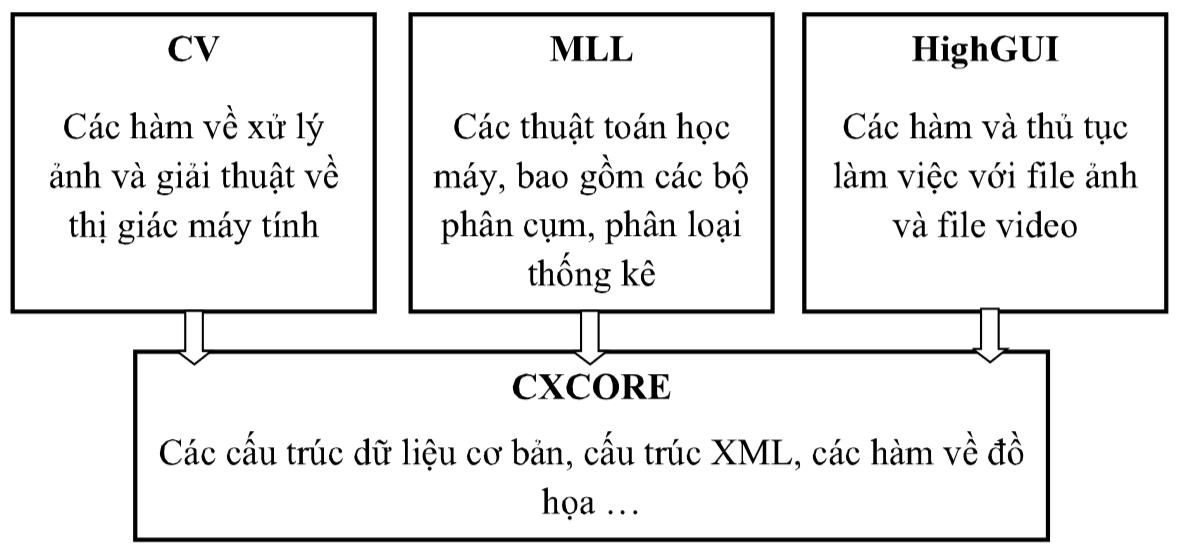
\includegraphics[width=0.99\linewidth]{Chapters/items/chap2_1.jpg}
        \caption{}
        \label{fig:chap2_1}
    \end{subfigure}
    \caption{Cấu trúc các phần của OpenCV.}
\end{figure}

Phần CV bao gồm các thư viện cơ bản về xử lý ảnh và các giải thuật về xử lý ảnh.
MLL là bộ thư viện về các thuật toán học máy, bao gồm rất nhiều bộ phân cụm và phân
loại thống kê. HighGUI chứa đựng những thủ tục vào ra, các chức năng về lưu trữ cũng
như đọc các file ảnh và video. Phần thứ 4, Cxcore chứa đựng các cấu trúc dữ liệu
cơ bản (ví dụ như cấu trúc XML, các cây dữ liệu …). Phần cuối cùng là CvAux, phần này
bao gồm các thư viện cho việc phát hiện, theo dõi và nhận dạng đối tượng (khuôn mặt, mắt …).

OpenCV - Python là một thư viện các ràng buộc Python được thiết kế để giải quyết các vấn đề
về xử lý ảnh và thị giác máy tính.

Python là ngôn ngữ lập trình có mục đích chung được bắt đầu bởi Guido van Rossum,
nó trở nên rất phổ biến rất nhanh trong thời gian gần đây, chủ yếu vì tính đơn giản
và khả năng đọc mã của nó. Nó cho phép lập trình viên thể hiện ý tưởng trong ít dòng
mã hơn mà không làm giảm khả năng đọc.

So với các ngôn ngữ như C/C++, Python chậm hơn. Điều đó nói rằng, Python có thể dễ dàng
được mở rộng với C/C++, cho phép chúng ta viết mã chuyên sâu tính toán trong C/C++
và tạo các trình bao bọc Python có thể được sử dụng làm mô-đun Python.
Điều này mang lại cho chúng ta hai lợi thế: thứ nhất, mã nhanh như mã C/C++ gốc
(vì đây là mã C++ thực tế hoạt động ở chế độ nền) và thứ hai, mã dễ dàng hơn trong
Python so với C/C++. OpenCV - Python là một trình bao bọc Python để thực hiện OpenCV C++
ban đầu.

OpenCV - Python sử dụng Numpy, một thư viện được tối ưu hóa cao cho các hoạt động số với
cú pháp kiểu MATLAB. Tất cả các cấu trúc mảng OpenCV được chuyển đổi sang và từ các mảng
Numpy. Điều này cũng giúp tích hợp dễ dàng hơn với các thư viện khác sử dụng Numpy
như SciPy và Matplotlib.



\section{Mô hình mạng neural tích chập (CNN - Convolutional neural network)}

Mạng neural tích chập (CNN) là một trong những mô hình học sâu tiên tiến phổ biến nhất và
có ảnh hưởng nhất với cộng đồng thị giác máy tính (Computer vision). CNN thường được dùng
trong các bài toán nhận dạng ảnh, phân tích ảnh, xử lý ngôn ngữ tự nhiên dưới dạng ảnh các bước sóng.
Và hầu hết đều cho hiệu quả tốt đến rất tốt.

CNN là một kiến trúc mạng neural sinh ra để xử lý các dữ liệu phi cấu trúc dạng ảnh. Có 2 loại lớp
chính trong CNN : lớp tích chập (Convolutional layer) và lớp gộp (Pooling layer)

\begin{figure}
    \begin{subfigure}{1.\textwidth}
        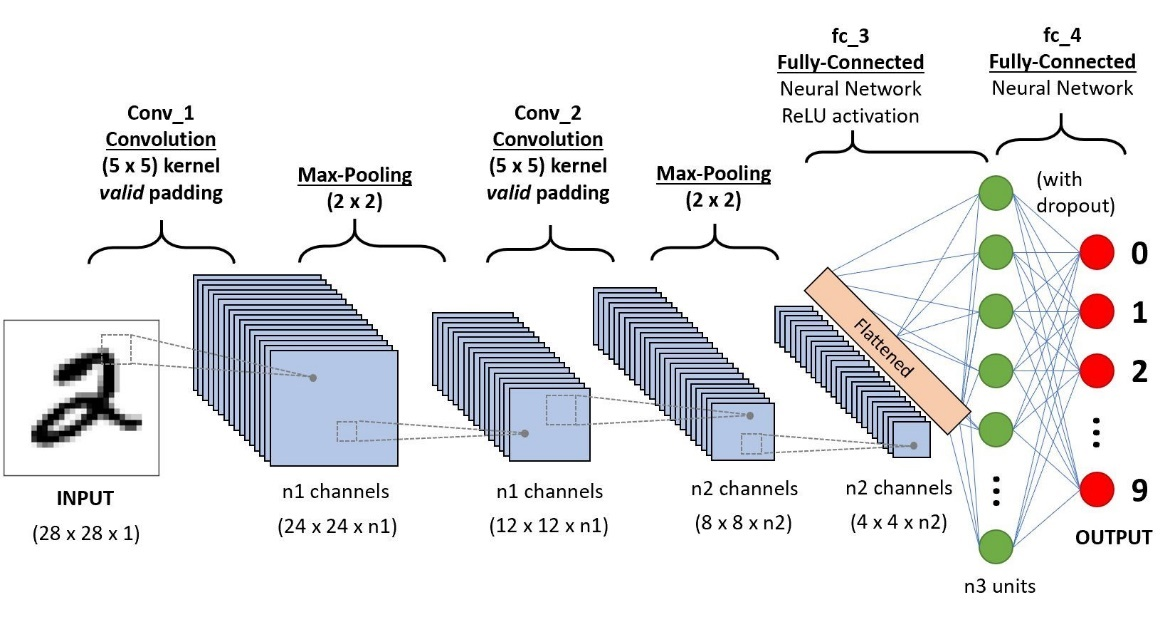
\includegraphics[width=1.\linewidth]{Chapters/items/cnn2_1.jpg}
        \caption{}
        \label{fig:chap2_2}
    \end{subfigure}
    \caption{CNN cho bài toán nhận diện chữ số.}
\end{figure}
\subsection{Lớp tích chập}

Lớp tích chập là lớp quan trọng nhất và thường cũng là lớp đầu tiên của của mô hình CNN. 
Lớp này có chức năng chính là phát hiện các đặc trưng có tính không gian hiệu quả. 
Trong tầng này có 4 đối tượng chính là: ma trận đầu vào, bộ lọc (filters) và trường thụ cảm, 
bản đồ đặc trưng (feature map). Lớp tích chập nhận đầu vào là một ma trận 3 chiều và một bộ lọc cần phải học. 
Bộ lọc này sẽ trượt qua từng vị trí trên bức ảnh để tính tích chập (convolution) 
giữa bộ lọc và phần tương ứng trên bức ảnh. Phần tương ứng này trên bức ảnh gọi là 
trường thục cảm (receptive field), tức là vùng mà một neuron có thể nhìn thấy để đưa 
ra quyết định, và mà trận cho ra bởi quá trình này được gọi là bản đồ đặc trưng (feature map). 

Để hình dung, có thể tưởng tượng, bộ filters giống như các tháp canh trong nhà tù quét 
lần lượt qua không gian xung quanh để tìm kiếm tên tù nhân bỏ trốn. 
Khi phát hiện tên tù nhân bỏ trốn, thì chuông báo động sẽ reo lên, giống như các bộ lọc 
tìm kiếm được đặc trưng nhất định thì tích chập đó sẽ cho giá trị tương ứng.

\begin{enumerate}
    \item Lớp tích chập được coi như xác định đặc trưng
    \item Các tham số : 
\end{enumerate}

\section{Máy dò khuôn mặt (Face detector)}
\section{Các kĩ thuật làm giàu dữ liệu (Data agumentation)}
\section{Mô hình học sâu được huấn luyện trước (Pre-train model)}
\subsection{Sử dụng mô hình được huấn luyện trước}
\subsection{Giới thiệu Facenet}
\subsection{Giới thiệu Mạng InceptionResnetV1}
\subsection{Kĩ thuật đánh giá bộ ba (Triplet loss)}

